\documentclass[10pt]{amsart} 
\usepackage{graphicx} 
\usepackage{float} % necessary for placement of figures
\usepackage{amsmath}
\usepackage{tikz}
\usepackage{pgfgantt} % load Gant chart package
\usepackage{array}
\usepackage[style = authoryear, sorting = nyt, backend = biber]{biblatex}
\addbibresource[location = local, type = file]{C:/Users/bloh356/Google Drive/Library/Library.bib}
% \addbibresource[location = local, type = file]{/Users/bloh356/Google Drive/Library/Library.bib}


\graphicspath {{figures/}}

\title{Uncertainty in reliability parameter estimates: Inclusion in the Generation Expansion Planning (GEP) problem}
\author{Andrew Blohm}
\date{\today}

\begin{document}
\maketitle

\section{Abstract}
What does uncertainty and nonstationarity in gas-fired generator reliability mean for the long-term reliability of our electricity system (and its optimal design)(In progress)? 
We anticipate that traditional methods significantly underestimate the riskiness of investment decisions and thus, overestimate system reliability, which potentially exposes consumers, generators, and system operators to greater risks of unmet demand. 
The contribution of our model to the literature is in the assessment of uncertainty and nonstationarity of the outage rate parameter on the optimal resource mix (as compared to existing methods). 
We anticipate that the composition, costs, and reliability resulting from our method will be quite different than existing methods, which rely on single point parameter estimates. 

\section{Introduction}
Investments in energy production capacity are subject to partial or complete irreversibility (i.e., large, sunk cost that is not particularly fungible) and are large, high-risk investments facing uncertain operating environments (i.e., economic and regulatory uncertainty)\parencite{bakirtzis:2012aa}. 
The Generation Expansion Planning (GEP) problem has been employed extensively to manage these risks while selecting an optimal production portfolio. 
The GEP model determines how best to meet expected future demand through the selection of plant size, production technology, and location, as well as timing over a planning horizon, usually between 10 - 30 years \parencite{hemmati:2013ab}. 
The GEP problem is well studied, from a variety of perspectives including: solution algorithms, incorporation of new production technologies, uncertainty characterization, reliability, time horizon, etc. \parencite{hemmati:2013ab}.
The GEP problem is a large-scale, highly-constrained mixed-integer linear program (MINLP) that requires complete enumeration (i.e., investigation of every combination of assets over the time horizon) to identify the global optimum \parencite{bakirtzis:2012aa}.  
The inability to undertake such an exercise has led to the development of simplifications to reduce the computational load of the problem. 

Two approaches are generally used to determine the solution to the GEP using micro-approach modeling: a centralized or decentralized approach \parencite{bakirtzis:2012aa}.\footnote{The micro-approach incorporates a high amount of model complexity that require operations research or meta-heuristic methods to solve but with the caveate that there is no guarantee that global optimality is achieved. Macro-modeling approaches reduce complexity by ignoring those features and constraints.} 
The centralized approach is appropriate in monopoly situations (i.e., a monopoly utility determining least cost expansion plans) or in deregulated markets by governing or regulating authorities to better design markets and policies \parencite{bakirtzis:2012aa}.
Solution methods for the centralized problem include stochastic dynamic programming (SDP)\parencite{}, non-linear programming (NLP)\parencite{}, evolutionary programming \parencite{}, multi-objective programming \parencite{}, mixed-integer linear programming (MILP) \parencite{}, in addition to other approaches \parencite{}\parencite{bakirtzis:2012aa}.  
[Insert the citations from \cite{bakirtzis:2012aa}.]
The decentralized approach accounts for the behavior of market participants, usually in a deregulated market framework \parencite{bakirtzis:2012aa}. 
For a more detailed discussion of the decentralized approach the reader is directed to \cite{bakirtzis:2012aa}. 

In this paper the centralized GEP problem is formulated as a \ldots

The proposed model is evaluated using the IEEE 14 and 30 bus test system \parencite{christie:2009aa}.\footnote{We downloaded the power system data for each of the 14, 30, 57, 188, and 300 bus test systems.}  
[Talk with Jeremy about the appropriate test system].
Of particular interest is how uncertainty is incorporated into the GEP model formulation, as well as the uncertainties that have thus far been considered. 
Uncertainty incorporation in the generation expansion planning problem has included price volatility, reliability of generation units, load forecast, electricity prices, and costs (i.e., fixed and variable) of each power production technology \cite{hemmati:2013ab, pereira2010decision, pereira2011generation}. 
A common approach to dealing with uncertainties in the GEP framework is Monte Carlo methods \parencite{pereira2010decision}.
Thus far 


Reliability in GEP problem formulation \ldots \parencite{hemmati:2013ab}. 

Two general approaches are used to assess power system adequacy: deterministic and probabilistic criteria. 
Deterministic criteria include a planning reserve margin, which could be one of several measures including, setting the reserve margin to the size of the largest generation unit, percentage of system capacity, etc. 
However, deterministic approaches (e.g., planning reserve margin) do not account for stochasticity in unit behavior, account for unit size, etc.
As a result, deterministic methods can lead to over-investment or inadequate system reliability \parencite{aghaei:2013aa}.

Instead, stochastic methods naturally account for randomness such as unit forced outage rates, size, etc. but at the expense of an increasing computational burden \parencite{aghaei:2013aa}.  
In general probabilistic metrics measure the duration, intensity or frequency in which demand exceeds the resources available at that time \parencite{dragoon:2006aa}.  	
The adequacy of the deployed resources to meet demand can be incorporated into the GEP problem using: Loss of Load Expected (LOLE)\footnote{The LOLE is the expected number of hours in which demand is not satisfied and is calculated as $LOLE = \sum_{k=1}^S P_k\left(C_T - L_k \right)\times t_k$, where there are S sub-periods and each sub-period is of length $t_k$.}, Loss of Load Probability (LOLP)\footnote{The LOLP is the long-run probability of power system demand exceeding the capacity available \parencite{endrenyi:1978}.  
LOLP can be calculated using daily peak load (i.e. hour demand for a 24 hour period) or using daily peak loads for a 1-year period using a load duration curve \parencite{endrenyi:1978}.}, Loss of Load Cost (LOLC), and Expected energy not served (EENS)\footnote{EENS is the expectation of the energy that the system is not capable of serving and is calculated as the following $EENS = P_k \left(C_T - L_k \right)\times \left(C_T- L_k \right)$.}.

Given it simplicity LOLE has been extensively used in the past, however, EENS does have certain advantages including that it encompasses the degree of the deficiency, as well as the likelihood \parencite[p622]{murugan2009nsga}.
Typically, the LOLE and EENS are generated using Monte Carlo techniques \parencite{billinton1996reliability, li2012uncertainty}. 
It is typically built recursively using the Capacity Outage Cumulative Probability Table (COCPT).\footnote{COCPT assumes that the failure of a unit is ``independent of the operating level, system load, and the outage pattern of other units'' (Goel presentation, 2011).} 


Assessing system adequacy using stochastic methods can lead to computational issues given the widely held belief that the GEP is actually a mixed integer non-linear program \parencite{aghaei:2013aa}.
As a result, several methods were developed to assess system adequacy.
\cite{} proposed the 'Z-Method' to evaluate system adequacy in the GEP problem, which replaces the stochastic adequacy assessment metric (i.e., loss-of-load probability (LOLP)) with a new constraint. 
The approach accounts for unit forced outage rates (FOR), system adequacy targets\footnote{In the GEP formulation framework the modeler would select an acceptable level of service (i.e., industry standard is an insufficient capacity with a frequency of 1-in-10 years)\parencite{}. 
The model would then calculate the appropriate reliability statistic using the EFOR (i.e., the number of hours of unit failure as a percentage of all available hours) for each generation unit type and size.}, uncertainty in expected load growth, as well as the size, type and number of units in the production mix \parencite{aghaei:2013aa, \ldots}. 

The goal of this paper is to formulate the GEP problem as a \ldots
The reliability metric (i.e., LOLE, LOLP, EENS, etc.) are highly sensitive to the EFOR parameter (i.e., a small change in the parameter estimate can lead to large changes in the reliability metric. 
GEP models have not explored the solution space that surrounds the EFOR parameter estimate. 

The rest of this paper is organized as follows: in the second section we propose the mathematical formulation of the \ldots [insert problem type] problem. 
The third section \ldots [solution algorithm discussion?]
In the fourth section we introduce our case studies before we discuss the results of our model formulation.
In the final section we discuss some relevant conclusions of our work. 

\section{\ldots Generation Expansion Planning problem formulation}
\subsection{Objective function \nopunct}

\subsection{Constraints \nopunct}
\subsubsection{Maximum construction limit \nopunct}
This constraint is a maximum allowable number, capacity, or investment amount for new generation sources to be built during period \textit{t} given limited resources (i.e., capital, manpower, space, etc.). 
\subsubsection{LOLP constraint \nopunct}
\begin{equation}
\textit{lolpc}_{t} \leq \textit{lolps}_{t} \forall t \in T 
\end{equation}

The $\textit{lolpc}_{t}$ is the loss-of-load probability at stage \textit{t} and $\textit{lolps}_{t}$ is the loss-of-load probability limit (i.e., the reliability target selected by the user) \parencite{dragoon:2006aa}. 
The equivalent Z constraint is \ldots


\subsubsection{Non-negativity constraints \nopunct}

\section{\ldots [Name of solution algorithm}


As a result, 
Planning and investment in power generation capacity expansion is difficult given the competing objectives for power producers (i.e. minimization of investment costs and maximization of reliability); uncertainty in a number of parameters (i.e.\ costs, demand, regulation), physical and technical constraints, complex mix of regulated and deregulated market structure across the country, and, large and lumpy investments, to name a few. 
One tool used in the long-term power planning process is Generation Expansion Planning (GEP) problem, which provides a framework to optimize generation investment.
	

To ensure that adequacy requirements (i.e., minimum level of service) are maintained the GEP problem formulation typically includes reliability constraints.\footnote{Reliability and adequacy are considered early in the planning process, typically well before stability and fault analysis. These factors are a necessary component of any long-term planning process; otherwise, there is no guarantee of having adequate supply to meet system demand.}\footnote{The determination of the adequate generation supply capacity can be divided into two areas: static and operating capacity requirements \parencite{billinton1984reliability}.
In this study, we focus on the static capacity requirement, which is the capacity that must be planned and installed in advance of system demand (i.e., as a part of a long-term planning process) \parencite{billinton1984reliability}.
Static capacity must be able to provide for outages and regularly scheduled maintenance, in addition to anticipated load growth \parencite{billinton1984reliability}.
Operating capacity, which we mention only for completeness, determines the capacity necessary to meet actual short-term load and is used in different frameworks, such as unit commitment problems \parencite{billinton1984reliability}.}
	 



\section{Methodology}
The generation expansion planning (GEP) model we present here is based upon a toy model presented in (Ehrenmann and Smeers 2011). We build upon the toy model through the inclusion of (i) multiple nodes, (ii) a complete transmission network, and (iii) stochastic demand, fuel inputs, and reliability. 
The individual generator is a price taking firm that maximizes profit by choosing an optimal capacity investment $(y_{hi})$ and generation $(x_{hli})$ given marginal costs of production $(C_h)$, electricity prices $(pi_{li})$, and investment costs $(I_{h})$.
Demand varies across the year using a load duration curve representation that decomposes annual demand into several load segments. 
In the next few sections we walk the reader through model development activities to date. 
Model development has proceeded incrementally to ensure the accuracy of results. 

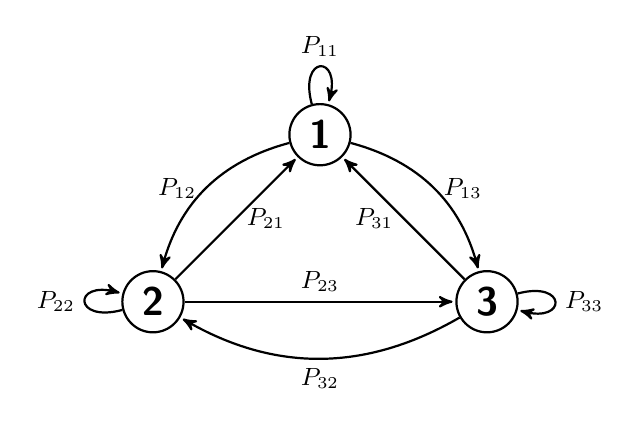
\begin{tikzpicture}[->,>=stealth',shorten >=1pt,auto,node distance=3cm,
                    thick,main node/.style={circle,draw,font=\sffamily\Large\bfseries}]
	\node[main node](1){1};
	\node[main node](2)[below left of=1]{2};
	\node[main node](3)[below right of=1]{3};

	\path[every node/.style={font=\sffamily\small}]
	 (1) edge [bend left] node[right] {$P_{13}$} (3)
	 edge [bend right] node[left] {$P_{12}$} (2)
	 edge [loop above] node[above] {$P_{11}$ }(1)
	 (2) edge node [right] {$P_{21}$} (1)
	 edge node [above] {$P_{23}$} (3)
 	 edge [loop left] node[left] {$P_{22}$} (2)
	 (3) edge node [left] {$P_{31}$} (1)
	 edge [loop right] node[right]{$P_{33}$} (3)	
	 edge [bend left] node[below]{$P_{32}$}(2);
\end{tikzpicture}

\subsection{Introduction}
	
	

	
	Addressing the inherent uncertainty of the EFOR parameter is a well studied problem even if the results aren't well incorporated into the typical GEP formulation. 
	A significant literature exists that has continued to evolve and incorporate advancements in other fields of study. 
	\cite{barbosa:1977}, Mohanta et al. (2007); Silva et al. (1988); Suhartono, Zika, and Sasaki (2000) treats the forced outage rates as a random variable with a certain mean and variance to approximate confidence limits around the LOLP. 
	Patton and Tram (1978) investigate sensitivities of reliability indices to variations in particular parameters in order to help planners identify the most important parameters and generators on the reliability indice. 
	Hamoud and Billinton (1981) use Fourier Transform methods to incorporate the uncertainty of parameters into the calculation of the LOLE index for a single area system. 
	Sahinoglu et al. (1983) derived probability density functions for the loss of load and unserved energy reliability indices using classical and Bayesian statistical inference. 
	Singh and Kim (1992) use a weighted composite of three gamma distributions (i.e., six parameter estimates) to generate a reliability probability distribution. 
	Billinton (1993) compares the accuracy and computing requirements of three analytical methods for computing reliability: load modification technique, cumulant method, and the segmentation procedure. 
	Noor and McDonald (1996) used expert elicitation and fuzzy set theory to estimate the forced outage rates of generating plants. 
	Oliveira, Melo and Pinto use Monte Carlo simulation methods to determine the effect of uncertainty in equipment reliability on composite reliability at the bus level. 
	Amjady and Ehsan (1999) use artificial neural networks in the estimation of forced outage rates. 

	Kim and Singh (2002) use fuzzy set theory to calculate the ?possibilistic? reliability indices based upon the uncertainty in the underlying data using the probability-possibility consistency principle algorithm. 
	Wu (2004) establishes a procedure for estimating Bayesian reliability in fuzzy environments (but doesn?t apply it to FOR).
	\parencite{mohanta:2005aa} Mohanta, Sadhu, and Chakrabarti (2005) uses a probabilistic Markov model in conjunction with fuzzy set theory to incorporate maintenance scheduling, failure-repair cycle, and aging of generating units in the generation of state probabilities. 
	Billinton and Li (2007) compare the EFOR (i.e., two state outage model) to a multi-state generator outage model in a composite system adequacy assessment. 
	Previous work has shown that the EFOR model can be overly pessimistic. 
	Chowdhury et al. (2007) incorporated uncertainty in the forced outage rate parameter of the generation adequacy assessment through a sensitivity analysis (varying the parameter 25% from the expected value).  
	Bhatkar et al. (2008) use fuzzy sets to incorporate data uncertainty into the calculation of the forced outage rate (and the well-being of the generating system).  
	Abdelfatah et al. (2011) determine trends in the hazard function while assessing the reliability of transformers in the Egyptian Electricity Transmission Company.
	Dent and Bialek (2011) model both random and systematic error in unit availability probabilities, which allows them to specify error bars around the reliability index produced. The authors show that small changes in the unit availability can lead to large changes in the reliability index.  
	Awadallah and Milanovic (2013) divide the uncertainty into aleatory (i.e., related to a random process) and epistemic (i.e., related to a lack of information) to quantify uncertainty representation (also have a good lit review). They use second order probability and evidence theory to quantify the uncertainty. 
	NERC 2014? uses a three stage technique to identify the reliability metrics under different modeling assumptions. 
	
	The world is changing around the electric power industry, as a result of changes in the domestic energy economy. 
	Much of the recently built and proposed power plants are either renewable or natural gas, which has made the power production sector the largest consuming sector of natural gas domestically \parencite{nerc2011gas}.
	Natural gas-fired growth is expected to increase by an average 1.3\% annual increase between 2012 and 2040 \parencite{eia2014annual}.\footnote{the information in this paragraph is from this article on eia today in energy http://www.eia.gov/todayinenergy/detail.cfm?id=17571\#} 
	By 2040, an additional 1,600 million megawatthours (MWh) of generation is projected to be available in the contiguous United States \parencite{eia2014annual}. 
	The changes in the electricity production mix are largely the result of environmental regulation and the increased domestic availability of natural gas, as a result of shale gas discoveries.
	The electricity production mix is phasing out coal-fired resources in favor of natural gas-fired resources, renewable energy resources (e.g. solar, wind, etc.), demand side management programs, and nuclear \parencite{nerc2011gads}. 
	For some regions (i.e., SERC and RFC), which cover portions of the southeastern and mid-western US, coal is expected to remain the largest generation source by fuel type \parencite{eia2014annual}.
	However, elsewhere much of the existing coal capacity retirements will be replaced by natural gas-fired resources \parencite{eia2014annual}.
	
	Gas-fired resources are particularly vulnerable to fuel supply disruptions as a result of characteristics of the gas pipeline industry, natural gas itself, and gas-fired generators. 
	(1) Natural gas is not easily stored on-site and as a result, real-time delivery of natural gas is necessary for plant operation \parencite{nerc2013gas}.
	(2) Gas-fired plants tend to have one connection to the pipeline network and as a result, are at risk from any disruptions in the connection \parencite{nerc2013gas}.
	(3) Gas-fired plants tend to have interruptible pipeline capacity contracts in place instead of firm capacity.
	Interruptible service is the lowest priority and can be interrupted for a number of reasons \parencite{nerc2013gas}.
	The increased demand is increasing the likelihood in some regions of pipeline capacity issues for natural gas-fired generation \parencite{nerc2013gas}.\footnote{The pipeline capacity expansion process is currently based on firm capacity only \parencite{nerc2013gas}. FERC will not provide the required certificate without sufficient firm capacity demand in place \parencite{nerc2013gas}. Thus, there exists a disconnect between the pipeline expansion mechanism and the rising demand for natural gas by electricity producers (this has been addressed in some regions by changes in contracting practices).}	
	Options are available to reduce the supply security risk (e.g.\ storage, firm fuel contracting, additional pipelines, dual-fuel capabilities, additional transmission lines, etc.) \parencite{nerc2011gas}.
	However, for many plants these options have not yet been implemented. 
	
	But is this actually an issue?
	In 2014, the Polar Vortex exposed previously unknown or underestimated energy security issues in the Northeastern United States. 
	Shutdowns were related to two factors: energy supply curtailment and ambient conditions resulting in forced outages or deratings (in particular during startup) \parencite{gugel2015polar}.
	Natural gas power plants were forced to shut down as a result of insufficient fuel supplies after there pipeline capacity was curtailed.
	During the worst of the polar vortex more than 35,000 MW of outages existed in the Eastern and Texas Interconnections \parencite{gugel2015polar}.  
	
	One issue with the existing literature is that it assumes the stationarity of the data. 
	The role of natural gas-fired generators is changing in the production mix (i.e., higher capacity factors) and more frequent ramping as a result of more renewables with unknown consequences on maintenance schedules and reliability [add citation].
	Generators are experiencing increasing O\&M costs as a result of increasing power plant cycling given larger deployments of variable generation, especially for plants designed as baseload units \parencite{nrel:2012aa}. 
	Cycling means operating the plant in response to system load requirements (i.e., load following, varying load levels, etc.); as opposed to operating it as a baseload resource \parencite{nerc:2012aa}.
	Each cycling exposes equipment to pressure and thermal stresses that can damage equipment and subsequently, lead to shorter component life expectancies, higher equivalent forced outage rates (EFOR), and shorter life expectancies \parencite{nerc:2012aa}. 
	 
	The natural gas industry is deploying more electric compressors throughout its pipeline system \parencite{nerc2011gas}. 
	And as a result of these changes, the natural gas and electricity generation industries are increasingly interdependent. 
	More natural gas fired plants means more exposure of the bulk power system to supply security issues (i.e.\ natural gas supply and delivery issues) \parencite{nerc2011gas}.
	Therefore, not only is there uncertainty in the EFOR parameter estimate but it might be changing.
	Changes in the domestic energy economy, as well as in the climate require additional techniques to identify the trends in the data and incorporate them in additional analyses (i.e., GEP).  
	
	The question put forward here is whether existing methods are capturing the true (and changing) risk to the bulk power system brought about by changes in the domestic energy economy. 
	By risk in this case, we mean specifically the ability to deliver electricity demanded with a certain reliability. 
	Uncertainty in GEP formulations tends towards uncertainty in load demands, fuel input prices, investment and operating costs, electricity prices, amongst others.
	\parencite{} demonstrated the importance of the forced outage rate (FOR) in generating the COCPT. 
	Shirvani (2012)[add citation] looked at the sensitivity of the EENS to the FOR through the COCPT and showed that it has a direct effect on the reliability of the system. 
	The FOR, defined as $FOR = \frac{\sum down time}{\sum down time + \sum up time}$ and EFOR are measures of unit unavailability (i.e. outage rates). 
	The FOR represents the availability of a unit across an entire period of time (e.g. a one-year period), while the EFOR is the availability of the unit during periods when the unit is needed.
	However, FOR provides a skewed sense of reliability given that we are more interested in the ability of a unit to meet demand when it is actually required to do so (Phoon, 2006, p19).  
	The North American Reliability Council (NERC) tracks the EFOR and FOR for in the Generating Availability Data System (GADS).
	
	We have not seen work dedicated to a sensitivity study of the equivalent forced outage rates (EFOR) on the LOLP.
	In particular, we have not seen work looking into the energy security concerns of the increasing gasification of the electricity production industry.
	First, we show that small changes in the EFOR can have large changes on the LOLP for a small toy system.
	A one percent change in the EFOR for each unit is associated with a \ldots change in the LOLP of the power system.
	Then we propose to incorporate uncertainty of the EFOR for gas-fired resources as a result of changes in the domestic energy economy using Bayesian methods.
	Next using the posterior density for the EFOR parameter we assess the range of LOLP for the PJM Interconnection region. 
	Finally, we discuss next steps. 
		
\subsection{Data}	
One approach would be to test the methods on the IEEE Reliability Test system \parencite{billinton:1994aa}. 
We use the IEEE Reliability Test System as an example system topology \parencite{}. 

	The changing electricity generation mix requires that industry personnel gain more experience with ``generating resource technology behavior, operating characteristics, and optimal planning approaches in order to properly assess reliability or improve performance analysis'' \parencite{nerc2011gads}. 
	Understanding the reliability and performance of existing and new production technologies is necessary to understand the reliability of the bulk power system in North America \parencite{nerc2011gads}. 
	It is also important to electric utilities since poor performing units can result in higher operating costs (i.e., loading units out of economic order), a need to purchase power, and/or installing additional capacity \parencite{}(GADS Introduction material).
	The industry, as a result, created the Generating Availability Database (GADs) as a means to share information on the causes and effects of unavailability, in addition to the development and improvement of strategies to prevent or mitigate availability losses that have proven useful to others \parencite{}(GADS intro material). 
	
	The North American Electric Reliability Corporation (NERC) compiles the Generating Availability Data System (GADS), which is an annual summary report for power stations located in the United States and Canada \parencite{nercgads}. 
	GADS contains information about the type of equipment used, performance characteristics, and descriptions of events (i.e. equipment failures). 
	Four types of events are reported in GADS: outages, deratings, reserve shutdowns, and non-curtailing events \parencite{gugel2015polar}. 
	It also contains data on the reliability, availability and maintainability of power plants (i.e., outage data). 
	The dataset includes the equivalent forced outage (EFOR), which is defined as the hours of unit failure (i.e. unplanned outage hours and equivalent unplanned derated hours) as a percentage of total available hours (i.e. unplanned outage, unplanned derated, and service hours)(wikipedia, GADS).\footnote{EFOR is calculated using IEEE Standard 762 definitions \parencite{gugel2015polar}.} 
	Outages can be divided into planned -- scheduled maintenance, versus unplanned outages -- unscheduled outages. 
	
	GADS began in 1979 as an extension of a data collection process that begin during the 1960s \parencite{}(GADS, The generating availability data system (GADS): Application and benefits, 1995).
	The database began as a voluntary with each participating utility providing detailed reports of each units operation and performance.
	However, since January 1, 2013, it is mandatory for conventional generating units with a nameplate capacity $\geq$ 20 MW to report reliability information to GADS \parencite{}(GADS frequently asked questions).  
	Variable energy sources are not required to report reliability information; a taskforce is currently underway to assess the best data collection methods for solar \parencite{}(GADS frequently asked questions). 
	The reports include quarterly information on the design information, types of outages and deratings, energy produced, fuel use, etc., which are then summarized in the annual \textit{Generating Availability Report} \parencite{} (GADS, The generating availability data system (GADS): Application and benefits, 1995).   
	It has involved to include data collection, data maintenance and support, in addition to data processing and reporting (i.e., trends in industry availability).
	
	The GADS contains operating histories for more than 7,700 generating units located in North America ($\approx$ 90\% of all installed generating capacity)\parencite{}(Generating Availability Data System: Data Reporting Instructions, 2015). 
	Events are defined as any time the operating status of a generator changes and include: outages, derates, reserve shutdowns, and non-curtailing events \parencite{}(Generating Availability Data System: Data Reporting Instructions, 2015).
	The event report will include informaiton on the event magnitude, primary cause, and, additional causes or components worked during the event \parencite{}(Generating Availability Data System: Data Reporting Instructions, 2015, pIII-2).
	In Figure \ref{fig:unit.states.GADS} we show the Unit States diagram from the \parencite{}(Generating Availability Data System: Data Reporting Instructions, 2015, pIII-5).
	

	Resources can first be categorized by whether they are active or inactive.
	Inactive resources are in one of three potential states: inactive reserve (IR), mothballed (MB), and, retired (RU). 
	An inactive reserve, mothballed, or retired unit is a unit whereby the unit is unavailable for an extended period of time for reasons unrelated to the equipment \parencite{}(Generating Availability Data System: Data Reporting Instructions, 2015, pIII-5). 
	Active states include: available and unavailable, which can be further broken down into unplanned outages and planned deratings for available resources, as well as unplanned outages and planned outages for unavailable resources \parencite{} (Generating Availability Data System: Data Reporting Instructions, 2015, pIII-6). 
	``An outage exists whenever a unit is not synchronized to the grid system and not in a reserve shutdown state. 
	An outage starts when the unit is either desynchronized from the grid or when it moves from one unit state to another (for example, goes from a reserve shutdown to a maintenance outage). 
	The outage ends when the unit is synchronized to the grid or moves to another unit state'' (Generating Availability Data System: Data Reporting Instructions, 2015, pIII-6). 
	
	In the GADS database an interruption in fuel supply, for example, as a result of interruptible supply of fuel as part of a fuel contract would be considered as events caused by external economic factors with a cause code 9131 \parencite{} (Generating Availability Data System: Data Reporting Instructions, 2015, Appendix B - pB-FS-29). . 
	
	The underlying data, used to calculate the annual summaries, is not publically available.
	Data sharing in GADS works via the following mechanism: an electric utility would share information for the types of power plants in its portfolio of assets.
	In GADS it would then have access to more detailed (and not publically available) reliability information concerning only those types of power plants.   
	The Generating Availability Report contains 17 categories of statistics for generating units and related equipment, which can be viewed at an annual or five-year cumulative basis. 
	The generating units are grouped by type, size (i.e., nameplate rating), and fuel (i.e., primary fuel used). 
	 
\subsection{Methods}
	We propose to use the GADS dataset to build a Bayesian regression model to estimate a posterior distribution around the EFOR parameter for each type (and size grouping) of power plant. 
	Reliability is known to be a function of or at least correlated with the size and type of power plant. 
	In our regression model we will control for confounding factors (i.e., weather, location, etc.) and trends (i.e., capacity factor, etc.) in the dataset.  
	
	Each generation unit can be represented by its capacity and its unavailability and each unit has only two states: on or an outage. 
	One disadvantage of the model is that it is a two-state system (i.e. up or down) while generating units are necessarily more complex in that they may experience partial failures in which they operate at reduced capacity levels (i.e. a 3- or even multi-state model).
	The capacity is a random variable in reliability analysis (Phoon, 2006, p19).
	\[
 	   P(X=x_i)=\left\{
             		   \begin{array}{c l}
             			   1-q & x_i = capacity_i \\
             			   q & x_i = 0
            		    \end{array}
         			\right.
	\]
	where, $q$ is the equivalent forced outage rate (EFOR)
	The capacity out of service then is multinomially distributed. 
	There are $2^n$ possible states, where $n$ is the number of generating units.
	And the likelihood of capacity greater than a particular value is $P(X \geq x_k) = \sum_{i \geq k} p(x_i)$.
	In other words, we sum all of the outcomes in which capacty exceeds a particular value and repeat this from the smallest unit capacity to the total system capacity value.  
	The likelihood of different capacity outages of the system, which is the basis of the COCPT. 			
	




\printbibliography
\end{document}

